%% MyServer
%% Copyright (C) 2008 Free Software Foundation, Inc.
%% This program is free software; you can redistribute it and/or modify
%% it under the terms of the GNU General Public License as published by
%% the Free Software Foundation; either version 3 of the License, or
%% (at your option) any later version.

%% This program is distributed in the hope that it will be useful,
%% but WITHOUT ANY WARRANTY; without even the implied warranty of
%% MERCHANTABILITY or FITNESS FOR A PARTICULAR PURPOSE.  See the
%% GNU General Public License for more details.

%% You should have received a copy of the GNU General Public License
%% along with this program.  If not, see <http://www.gnu.org/licenses/>.

\documentclass[12pt]{article}
\usepackage{epsfig}
\usepackage{url}
\usepackage{fancyhdr}
\usepackage{listings}
\usepackage{color}
\definecolor{commentsRGB}{rgb}{0.13,0.55,0.13}
\definecolor{stringsRGB}{rgb}{0.63,0.125,0.94}


\lstloadlanguages{C++}

\lstset{
keywordstyle = \color{blue},
identifierstyle =, 
commentstyle = \color{commentsRGB}, 
stringstyle = \ttfamily \color{stringsRGB},
language = {C++},
extendedchars = true, 
breaklines = true,
breakautoindent = true,
breakindent = 30pt,
}


\date{}
\author{}
\title{GNU MyServer hacking guide}

\begin{document}
\maketitle

\begin{figure}[H]
  \begin{center}
    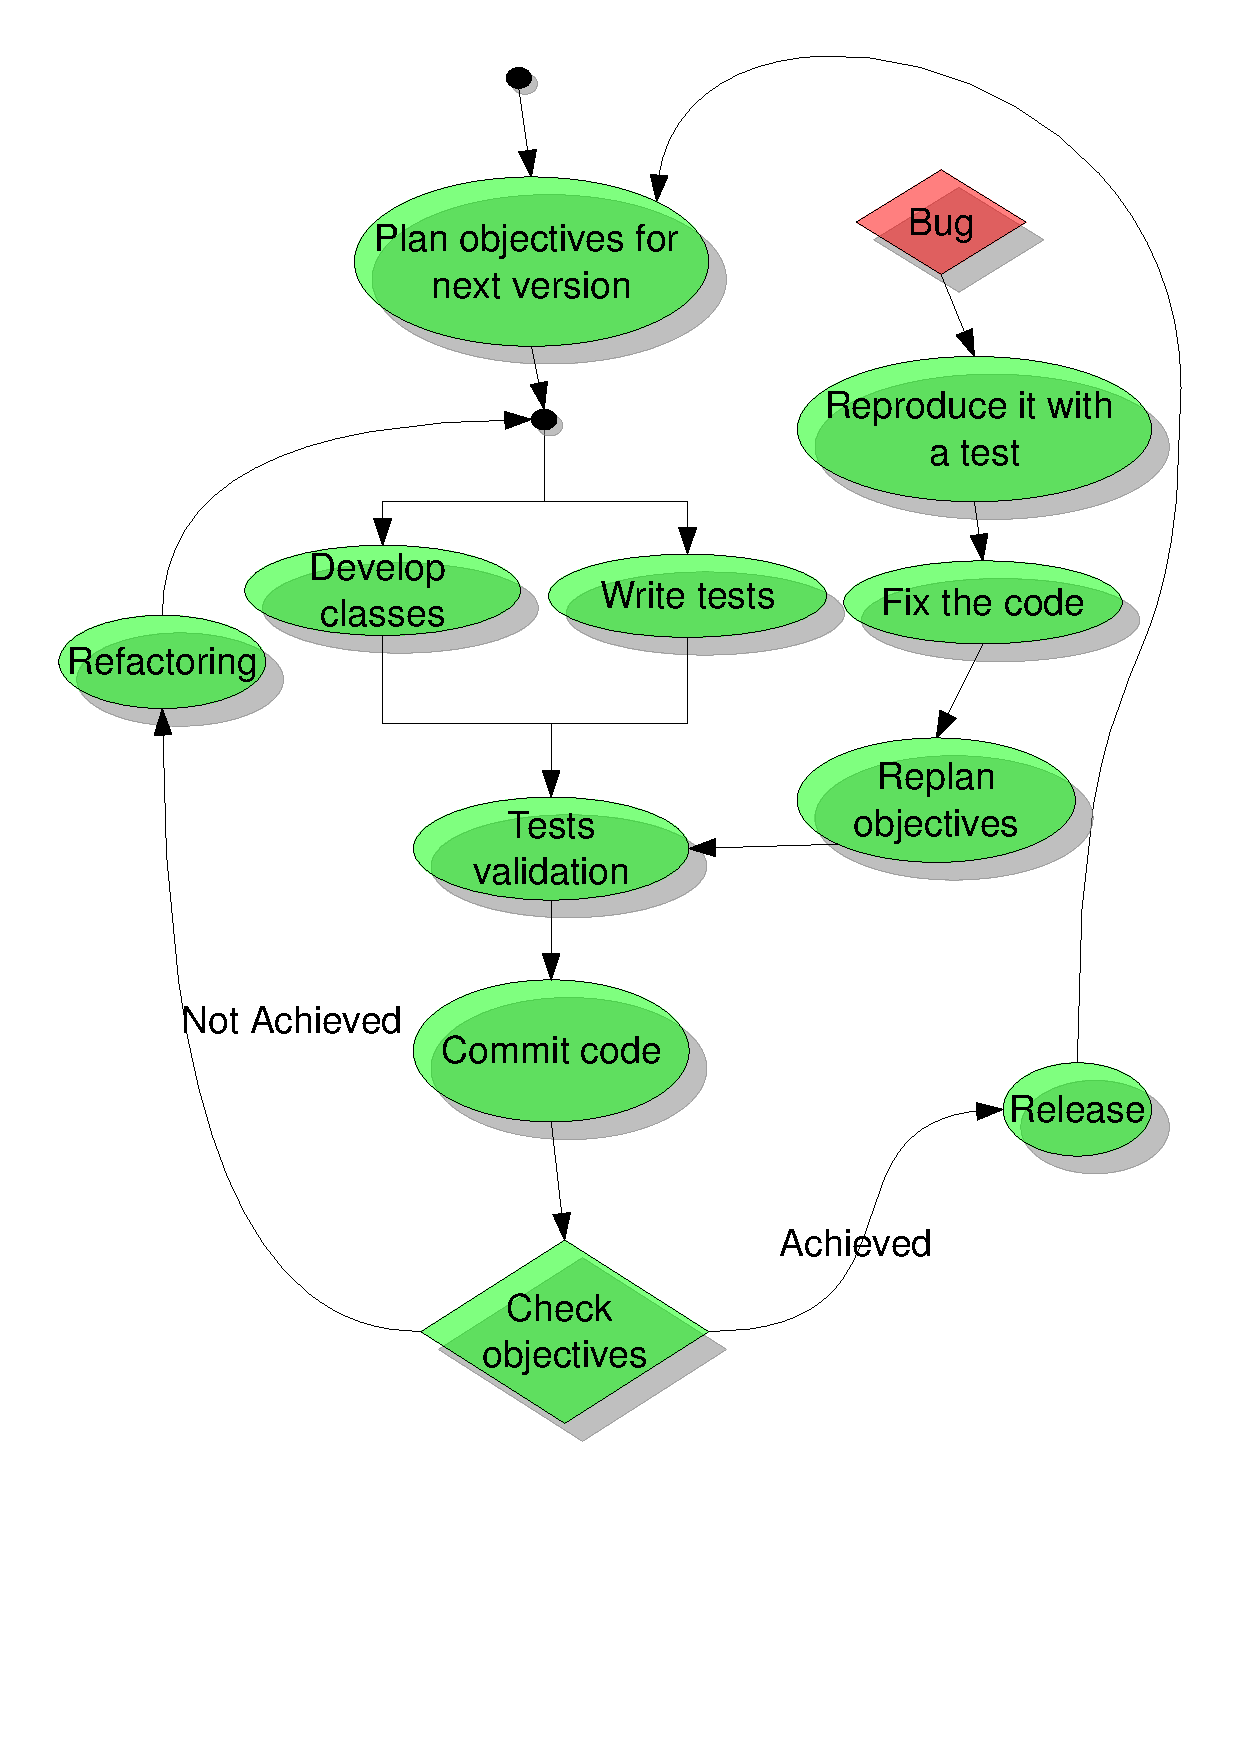
\includegraphics[height=0.9\textheight]{dev_scheme}
  \end{center}
  \caption{Development process}
  \label{figure:dev_proc}
\end{figure}

\begin{section}{Introduction}
This document is an introduction to how develop GNU MyServer and
interact with other team members.
It is not and it doesn't want to be a complete guide to be a
programmer but only an introduction to the development model used by
this project.
The figure \ref{figure:dev_proc} shows the GNU MyServer development
process.
In short, at every loop some objectives are planned and a new release
will be out when they will be completed.
Before the final release is completed, some minors releases are done
on specified dates, no matter if planned objectives are already
completed or not.

This development model is not test-driven because write tests and
develop code are parallel processes.
If somebody finds test-driven a better choice then he or she is free
to adopt it, it is a personal choice, in any case code is committed
to the central repository after it is compilable and it is validated
by all tests.
The central repository at any time must contain a snapshot of the
current development status and it must be compilable and usable.

Differently the bugs fixing process is test driven, when a bug is
detected it should be reproduced by a test.  After the code is
modified to validate all tests, including the new bug test.
Objectives are replanned after a bug is fixed because there can be
need to release immediately.

Before the release, code can be changed until it reaches a good
readable status (refactoring).
\end{section}

\begin{section}{How start hacking}
The first step to take before be a MyServer hacker is to fetch latest
source code version from the subversion version(section
\ref{section:svn}) and be able to compile it, only after you are able
to compile and execute MyServer you can think about modify its source
code.
To be updated about the MyServer development the best idea is to join
the mailing lists (section \ref{section:ml}), it is not required to
partecipate actively there, reading what other members are discussing
is a good way to be introduced to the project; hopefully after some
time you will be very active there too.
\end{section}

\begin{section}{Tasks list}
The file TODO in the GNU MyServer directory root contains a list of
tasks that need to be completed.
Each entry in the TODO list should be a basic task, in a way that a
developer without a previous knowledge of the software can start
working immediately on it.

In the past the TODO list files used to be a wish list with tasks like
\textit{``Implement the FTP protocol''}, such big tasks must be
avoided and replaced by smaller and more detailed ones, that can be
done in few hours.
Have these macro-tasks means that the feature is not well designed or
not designed at all and it is a good idea to plan a design for it
before start working on its implementation and discuss it on the
mailing list with other team members.
Lately it will be possible to define small tasks and proceed with its
implementation.
\end{section}

\begin{section}{Source code guidelines}

\begin{subsection}{License header}
Any source file must start with the GPL license header.  All the
source code is copyrighted to the \textit{Free Software Foundation
  Inc.}
You can take the header directly from existing source files.
\end{subsection}
  
\begin{subsection}{Code format}
This simple code snippet shows how format the code and how indent it.
Don't use the tab character to indent it, instead use 2 blank spaces. 
\begin{lstlisting}{language=C++}
//include/foo.h
class Foo
{
public:
  Foo(){}
  int max(int a, int b)
  {
    if(a > b)
      return a;

   return b;
  }
  int longMethod();
private:
  int bar;
};
....
//src/foo.cpp
int Foo::longMethod()
{
...
  return bar;
}
\end{lstlisting}
\end{subsection}

\begin{subsection}{Writing code suggestions}
These are some simple rules to keep in mind writing code:
\begin{itemize}
\item Short methods, avoid long methods.
\item Add comments only when there is really need, code should be
  clean itself, have many comments will make it more difficult to
  maintain because any change in the code must be duplicated in the
  comment.
\item Add a doxygen compatible comment to every method, this is the
  only kind of comment that should be always present, more information
  about doxygen can be found here:
  \url{http://www.stack.nl/~dimitri/doxygen/}.
\item Try to avoid mock objects during testing, base classes can be
  implemented to don't do anything, if you don't know what a mock
  object is then take a look
  here~\url{http://en.wikipedia.org/wiki/Mock_object}.
\item Possibility to use unit testing as code snippets for APIs, tests
  code should be as much clean and readable as possible.
\item Make the code breathe, add blank lines to separe different
  sections and make it clearer.
\end{itemize}
\end{subsection}
In general any \textit{code smell} should be considered too, you can
find some of them here: \url{http://c2.com/cgi/wiki?CodeSmell}.
\end{section}
\clearpage

\begin{section}{Mailing lists}\label{section:ml}
The communication with other project members is fundamental and when a
message interests everybody then it should be sent on the dev mailing
list, you can find a list of the mailing lists
here:~\url{http://savannah.gnu.org/mail/?group=myserver}.

Actually there are two mailing lists:
\begin{itemize}
\item \textit{bug-myserver@gnu.org} Differently from what the name can
  suggest, it is not used only for bugs but for any development
  related discussion.
\item \textit{myserver-commit@gnu.org} It is a read-only mailing list,
  any commit to the repository is notified here.  It is not only a way
  to annouce you that something happened but it has a very important
  role in the development process.  Review patches by humans is done
  at this point, after the commit happened, more eyes can notice
  better if something is wrong.  If you notice that something is not
  as it should be, then reply to the \textit{bug-myserver@gnu.org}
  adding the developer who made the commit in CC, explaining what you
  consider wrong.
\end{itemize}
\end{section}

\begin{section}{Subversion repository}\label{section:svn}
\begin{subsection}{Branches}
If there is need to change many things in the source code, like for
example when we implemented an event driven scheduler, that changed
several classes in different sections of the code, then it is a good
choice to create a branch from \textit{trunk}.
After the job is completed in a way the branched version is working
well and it is validated by tests then it can be merged back to the
\textit{trunk} tree.
For branches it is not valid the rule that it should work at any time
or validated by tests as they are experimental versions.  In general
the developer who created the branch is responsible for the politic to
follow.
\end{subsection}

\begin{subsection}{Access the repository}
You can find information about how access the source code repository here:
\url{http://savannah.gnu.org/svn/?group=myserver}.
\end{subsection}

\begin{subsection}{Commits}
A commit to the repository shouldn't contain two or more different
modifications to the source code.
Every commit must be logical different than other ones, any different
modification must stay in a different commit.
Use a short but descriptive commit message, they ChangeLog file is not
maintained manually as it is possible to retrieve it using the commits
history.  The \textit{svn2cl} utility can generate a GNU compatible
ChangeLog file.
\end{subsection}
\end{section}

\end{document}
